% =====================================================================
%  N5: the inverse-modelling workflow.
%  Build: pdflatex fig_inverse.tex && cp fig_inverse.pdf figures/N5_inverse_workflow.pdf
% =====================================================================
\documentclass[border=4pt]{standalone}
\usepackage[T1]{fontenc}
\usepackage{helvet}
\renewcommand\familydefault{\sfdefault}
\usepackage{tikz}
\usetikzlibrary{arrows.meta,positioning,calc,fit,backgrounds}

\definecolor{ohqblue}{HTML}{1F5C8B}
\definecolor{ohqteal}{HTML}{2A9D8F}
\definecolor{ohqrust}{HTML}{E76F51}
\definecolor{ohqgrey}{HTML}{6B7280}
\definecolor{bandfill}{HTML}{EDF1F4}

\begin{document}
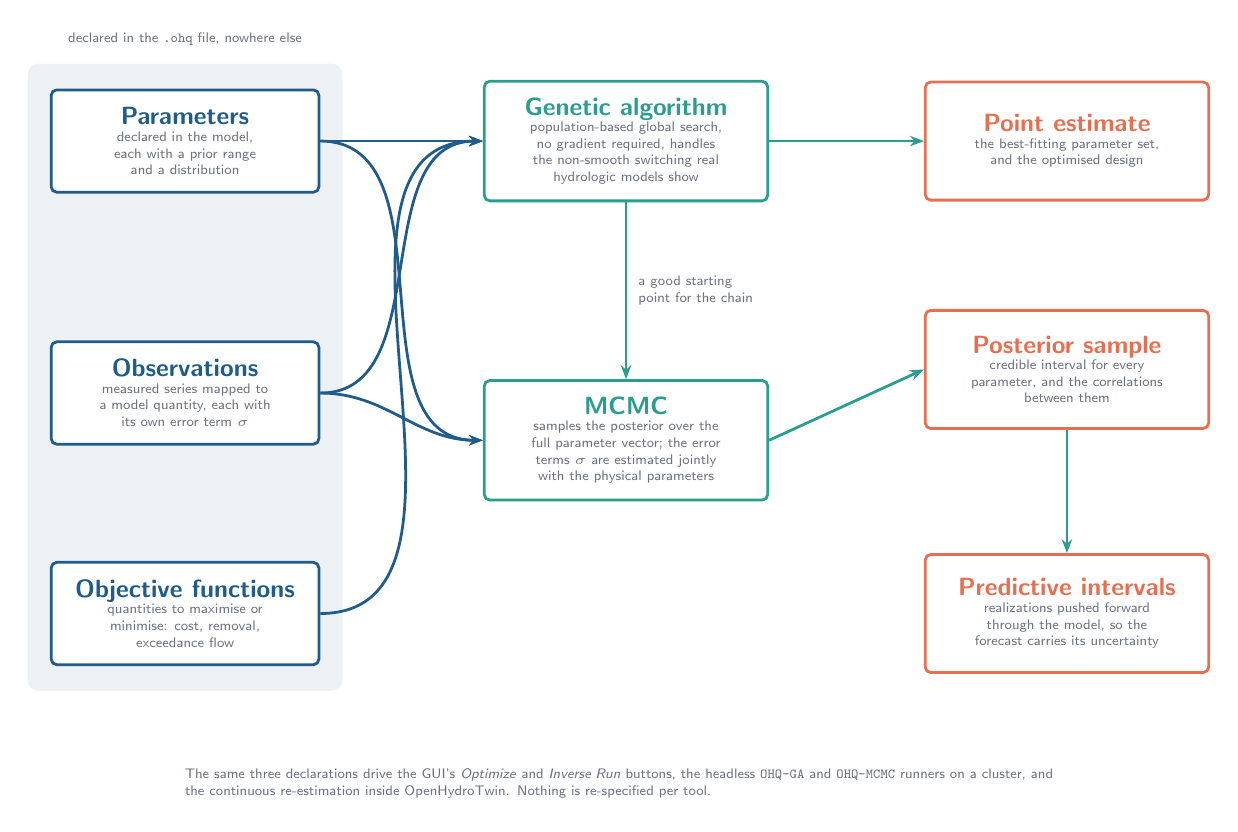
\begin{tikzpicture}[
  font=\sffamily,
  inp/.style={draw=ohqblue, line width=1pt, fill=white, rounded corners=2pt,
              align=center, inner sep=6pt, font=\tiny, text=ohqgrey,
              minimum width=34mm, minimum height=13mm},
  eng/.style={draw=ohqteal, line width=1pt, fill=white, rounded corners=2pt,
              align=center, inner sep=6pt, font=\tiny, text=ohqgrey,
              minimum width=36mm, minimum height=15mm},
  res/.style={draw=ohqrust, line width=1pt, fill=white, rounded corners=2pt,
              align=center, inner sep=6pt, font=\tiny, text=ohqgrey,
              minimum width=36mm, minimum height=15mm},
  arr/.style={-{Stealth[length=5pt]}, ohqblue, line width=1pt},
  arrt/.style={-{Stealth[length=5pt]}, ohqteal, line width=1pt},
  lbl/.style={font=\tiny, text=ohqgrey, align=center, inner sep=2pt},
]
\def\hb#1{\textbf{\color{ohqblue}\small #1}}
\def\hteal#1{\textbf{\color{ohqteal}\small #1}}
\def\hr#1{\textbf{\color{ohqrust}\small #1}}

% ---------------- inputs -------------------------------------------
\node[inp] (par) at (0, 1.6)
  {\hb{Parameters}\\declared in the model,\\each with a prior range\\and a distribution};
\node[inp] (obs) at (0,-1.6)
  {\hb{Observations}\\measured series mapped to\\a model quantity, each with\\its own error term $\sigma$};
\node[inp] (objf) at (0,-4.4)
  {\hb{Objective functions}\\quantities to maximise or\\minimise: cost, removal,\\exceedance flow};

% ---------------- engines ------------------------------------------
\node[eng] (ga) at (5.6, 1.6)
  {\hteal{Genetic algorithm}\\population-based global search,\\no gradient required, handles\\the non-smooth switching real\\hydrologic models show};
\node[eng] (mc) at (5.6,-2.2)
  {\hteal{MCMC}\\samples the posterior over the\\full parameter vector; the error\\terms $\sigma$ are estimated jointly\\with the physical parameters};

% ---------------- outputs ------------------------------------------
\node[res] (pt) at (11.2, 1.6)
  {\hr{Point estimate}\\the best-fitting parameter set,\\and the optimised design};
\node[res] (po) at (11.2,-1.3)
  {\hr{Posterior sample}\\credible interval for every\\parameter, and the correlations\\between them};
\node[res] (pr) at (11.2,-4.4)
  {\hr{Predictive intervals}\\realizations pushed forward\\through the model, so the\\forecast carries its uncertainty};

% ---------------- flow ---------------------------------------------
\draw[arr] (par.east) -- (ga.west);
\draw[arr] (obs.east) to[out=0, in=180] (ga.west);
\draw[arr] (objf.east) to[out=0, in=180] (ga.west);
\draw[arr] (par.east) to[out=0, in=180] (mc.west);
\draw[arr] (obs.east) to[out=0, in=180] (mc.west);

\draw[arrt] (ga.east) -- (pt.west);
\draw[arrt] (ga.south) -- node[lbl, right, xshift=2pt, align=left]
  {a good starting\\point for the chain} (mc.north);
\draw[arrt] (mc.east) -- (po.west);
\draw[arrt] (po.south) -- (pr.north);

% ---------------- framing ------------------------------------------
\begin{scope}[on background layer]
  \node[fill=bandfill, rounded corners=4pt, fit=(par)(objf), inner xsep=8pt,
        inner ysep=9pt] (inb) {};
\end{scope}
\node[lbl, anchor=south] at ([shift={(0,4pt)}]inb.north)
  {declared in the \texttt{.ohq} file, nowhere else};

\node[lbl, anchor=north, text width=112mm, align=left] at (5.6,-6.3)
  {The same three declarations drive the GUI's \emph{Optimize} and
   \emph{Inverse Run} buttons, the headless \texttt{OHQ-GA} and
   \texttt{OHQ-MCMC} runners on a cluster, and the continuous
   re-estimation inside OpenHydroTwin. Nothing is re-specified per tool.};

\end{tikzpicture}
\end{document}
